\documentclass[11pt]{article}
\usepackage[utf8]{inputenc}
\usepackage[english]{babel}
\usepackage{amsmath}
\usepackage{amsfonts}
\usepackage{dsfont}
\usepackage{graphicx}
\usepackage{float}
\usepackage{lipsum}
\usepackage{multicol}
\usepackage{xcolor}
\usepackage{tabularx}
\usepackage{booktabs}
\usepackage{hyperref}
\usepackage{wrapfig}
\usepackage{listings}
\usepackage{booktabs}

\newcolumntype{Y}{>{\centering\arraybackslash}X}
\usepackage[left=2.00cm, right=2.00cm, top=2.00cm, bottom=2.00cm]{geometry}

\title{AN2DL Reports Template}

\begin{document}
    
    \begin{figure}[H]
        \raggedright
        
\includegraphics[scale=0.4]{figures/polimi.png} \hfill 
\includegraphics[scale=0.3]{figures/airlab.jpeg}
    \end{figure}
    
    \vspace{5mm}
    
    \begin{center}
        % Select between First and Second
        {\Large \textbf{AN2DL - Second Homework Report}}\\
        \vspace{2mm}
        % Change with your Team Name
        {\Large \textbf{DeepL}}\\
        \vspace{2mm}
        % Team Members Information
        {\large Matteo Bonfadini,}
        {\large Elena Lippolis,}
        {\large Lorenzo Cossiga,}
        {\large Michele Baggi}\\
        \vspace{2mm}
        % Codabench Nicknames
        {matteobonfadini,}
        {elenalippolis1,}
        {lorenzocossiga,}
        {Miki\_Polimi}\\
        \vspace{2mm}
        % Matriculation Numbers
        {243786,}
        {252310,}
        {242309,}
        {252119}\\
        \vspace{5mm}
        \today
    \end{center}    
    %\vspace{5mm}

    \begin{multicols*}{2}

    %\noindent Here our \emph{DeepL-2} work.

    \section{Introduction} % (fold)
    \label{sec:introduction}
    
    The project aims to perform \emph{semantic segmentation} on \(64 \times 128\) grayscale images of Mars terrain. This is a challenging task in \textbf{computer vision}, since the goal is:
    \begin{equation*}
    \boxed{
    \begin{gathered}
    \text{Given an image }I,\text{ associate to each pixel }p \\
    \text{ a label from }C 
    \end{gathered}
    }
    \end{equation*}

    \noindent where $C$ is the set of labels. The result of segmentation is a map of labels containing in each pixel the estimated class \cite{SSslide}.

    In recent years, semantic segmentation performance has been greatly improved using \textbf{deep learning techniques} \cite{semsegm}. In this paper, we illustrate how we developed from scratch a \emph{neural network} capable of generating accurate segmentation masks of Mars terrain. Our approach involves pre-processing the dataset by removing outliers, addressing class imbalance through targeted augmentation techniques, and implementing a U-Net model, an idea firstly introduced for biomedical applications in \cite{originalUnet}, to enhance segmentation performance.
    
    % section introduction (end)

    \section{Problem Analysis} % (fold)
    \label{sec:problem_analysis}
    
    The given dataset consists of:
    \begin{itemize}
        \item A \textbf{training dataset} of 2615 segmented images from Mars terrain. Each image is paired with a mask representing the class of each pixel, as shown in Figure~\ref{fig:mars1}.

        \item A \textbf{test dataset} of 10022 unlabeled test images.
    \end{itemize}

    \begin{figure}[H]
            \centering
            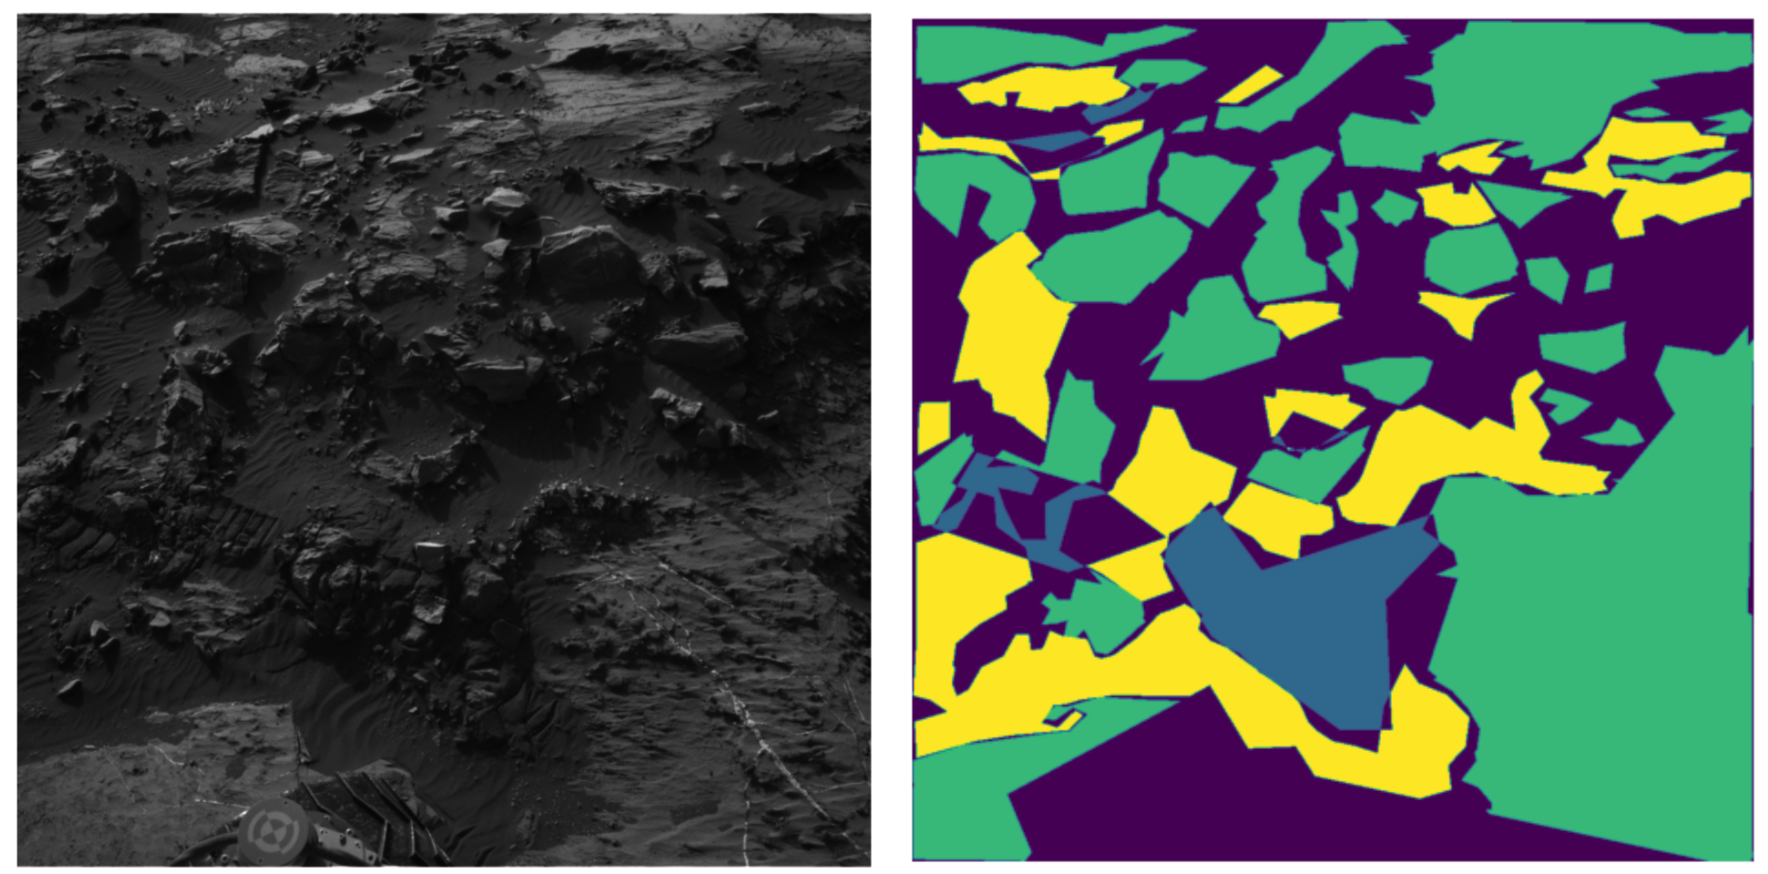
\includegraphics[width=0.85\linewidth]{figures/mars1.png}
            \caption{Example pair of image and mask.}
            \label{fig:mars1}
    \end{figure}

    \noindent Figure~\ref{fig:palette} shows for each color of image on the right the specific class $c$ from the labels set $C$. We emphasize the importance of the background class, as in real-world images -including the case of Mars terrain - certain regions may not belong to any predefined class. Without a background class, the model could become \emph{confused}, resulting in misclassifications.
    
    \begin{figure}[H]
            \centering
            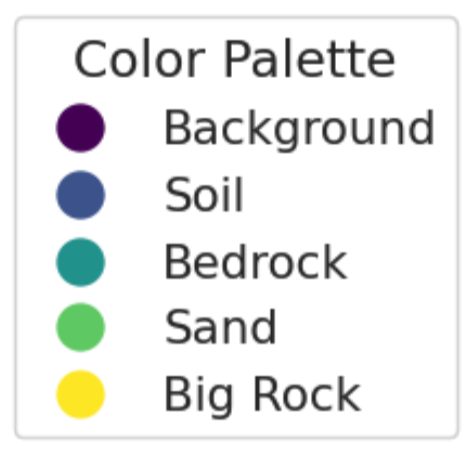
\includegraphics[width=0.35\linewidth]{figures/mars_palette.png}
            \caption{Viridis colormap of the set $C$.}
            \label{fig:palette}
    \end{figure}
    
    \noindent We tackled the segmentation problem in a 3-phase approach.

    \subsection{Phase 1: Data Inspection}

    We began by inspecting the dataset and visualizing several image-mask pairs. During this process, we noticed a few anomalous images, which we refer to as \emph{alien} images, scattered throughout the training data. Since these were clear \textbf{outliers} that could potentially disrupt the learning process, we sought an efficient method to identify them.
    
    To define what constitutes an \emph{alien} in our dataset, we analyzed two image properties: the mean pixel value and pixel variance. By comparing these metrics to carefully chosen threshold values, we successfully detected approximately 100 alien images.
    
    While fine-tuning the thresholds, we observed an interesting pattern: all alien images shared the same mask, regardless of variations in the background. Leveraging this observation, we refined our detection method by comparing the labels across images, enabling us to identify and remove a total of 110 alien images.

    \subsection{Phase 2: Class Imbalance and Loss function}

    Figure~\ref{fig:freq} presents the frequency of each class in the dataset, expressed as a percentage of the total number of labels, along with their corresponding category descriptions.

    \begin{figure}[H]
    \centering
    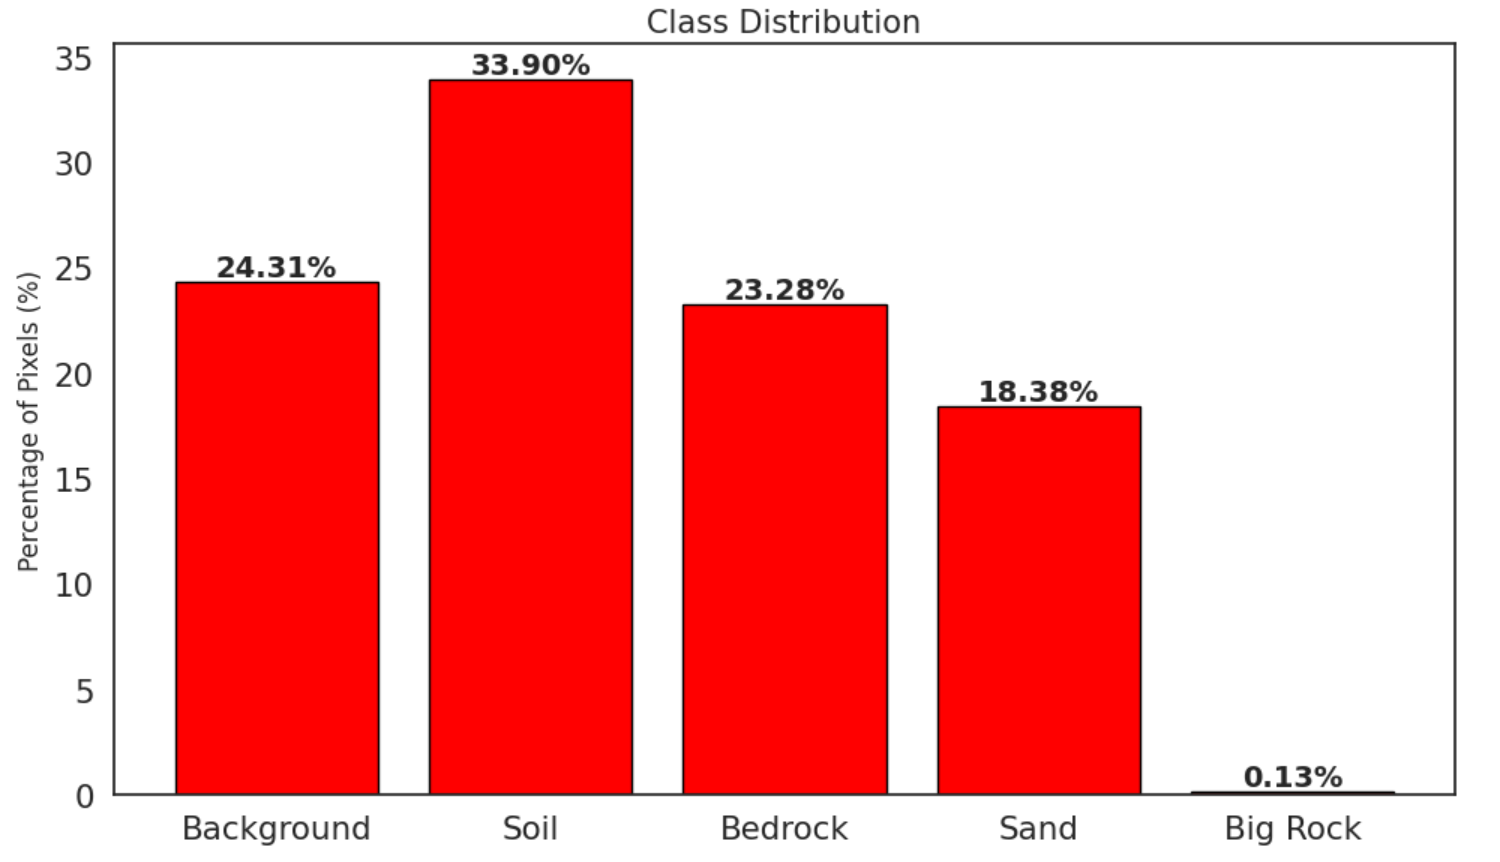
\includegraphics[width=0.8\linewidth]{figures/freq.png}
    \caption{Class frequencies in the dataset, expressed as percentages.}
    \label{fig:freq}
    \end{figure}
    
    \noindent Our dataset exhibits a significant class imbalance, with the Big Rock class comprising only 0.13\% of the data. \textit{Focal Loss} addresses this by emphasizing harder-to-classify, minority samples. The background class is excluded from weighting, allowing greater focus on rare classes like Big Rock, which is assigned higher importance due to its infrequency.

    \subsection{Phase 3: UNet Architecture}

    For the main part of the segmentation task, we started from the UNet model described during exercise class \cite{unet}. This design has the potential to effectively captures both global context and fine-grained details, making it highly suited for handling complex regions in Mars terrain images.

    % section problem_analysis (end)

    \section{Method} % (fold)
    \label{sec:method}

    We present here two models created from the baseline code mentioned before. They both were evaluated according to the mean intersection over union metric, computed as:
    \begin{equation*}
    \frac{1}{C}\sum_{c\in C}\frac{\mathbb{I}(y=c)\wedge \mathbb{I}(\hat y=c)}{\mathbb{I}(y=c)\vee \mathbb{I}(\hat y=c)}
    \end{equation*}

    given the set of classes, the ground truth, and the model predictions.

    \subsection{Advice-based Model}

    The pre-processing pipeline includes \emph{loading}, \emph{resizing}, and \emph{normalizing} images and labels to the range $[0,1]$, along with \emph{category mapping} and \emph{data augmentation} (e.g., random horizontal flips).
    
    Then, the baseline UNet architecture is shown in Figure~\ref{fig:U}. It features a straightforward \emph{encoder-decoder} structure where the encoder extracts hierarchical features using convolutional blocks and pooling layers, while the bottleneck captures abstract features with the highest number of filters. The decoder reconstructs spatial dimensions with upsampling layers and skip connections, and the final Conv2D layer outputs a multi-class segmentation map with softmax activation.

    \begin{figure}[H]
    \centering
    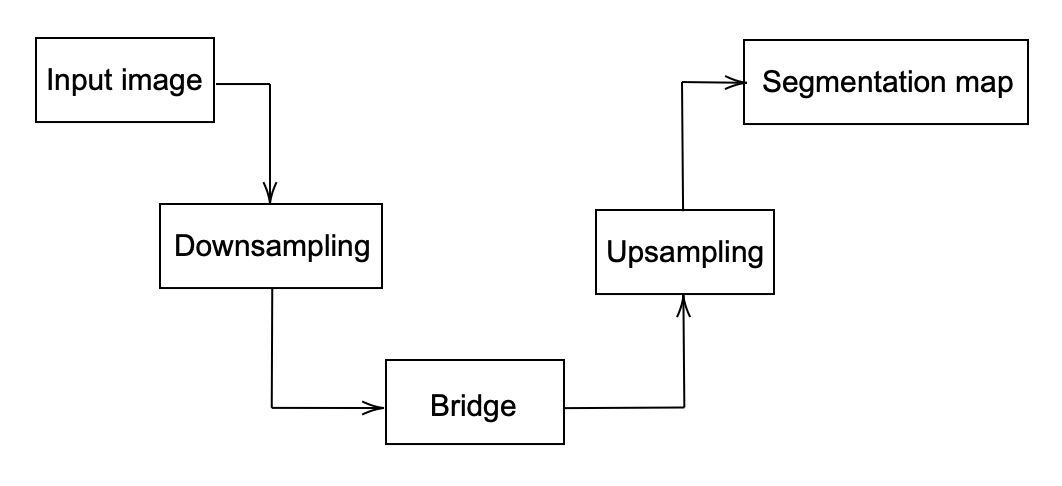
\includegraphics[width=0.9\linewidth]{figures/U.png}
    \caption{Overview of the UNet architecture.}
    \label{fig:U}
    \end{figure}
    
    \noindent We then enhanced the model by following all the advices given by Professor Lomurno. Firsty, we  introduced \textbf{residual connections} in the \emph{bottleneck} to stabilize gradients and improve learning efficiency.

    We employed a multiple \textit{loss function} incorporating the categorical crossentropy (\texttt{ce}), the dice loss (\texttt{dc}), the focal loss (\texttt{fc}) and the boundary loss (\texttt{bd}) to improve model performance. We combined these losses with specific weights to balance their contributions effectively:
    \begin{equation*}
    \text{Combined Loss} = 0.4 \cdot \texttt{ce} + 0.3 \cdot \texttt{dc} + 0.2 \cdot \texttt{fc} + 0.1 \cdot \texttt{bd}
    \end{equation*}

\noindent Finally, a dual UNet framework was implemented to integrate large-scale and fine-detail segmentation with scale-weighted losses. The bottleneck was further improved with \emph{parallel dilated convolutions}, \emph{squeeze-and-excitation mechanisms}, and \emph{global context modules} to maximize feature fusion. We implemented \emph{deep supervision} with weighted intermediate losses at various decoder levels to refine predictions and further improve gradient flow. 

\emph{Group normalization} replaced \emph{batch normalization} in the upsampling layers because it resulted in being less sensitive to batch size and capturing fine details, improving the overall segmentation performance. \emph{Skip connections} were enhanced through weighted fusion mechanisms with learnable parameters, such as gated mechanisms. 

Multi-scale contextual awareness was achieved through \emph{dilated convolutions} and \emph{pyramid pooling}, with varying dilation rates to balance local detail and global context, and \emph{transformer blocks} were integrated into the architecture to capture long-range feature dependencies, while \emph{adaptive feature fusion} was enabled through trainable gates. A dynamic learning rate adjustment strategy was adopted using a \emph{warm-up phase} followed by a \emph{cosine annealing scheduler} to balance exploration and convergence during training. 

We also developed post-processing network to analyze the background class, and channel attention mechanisms, including \empg{squeeze-and-excitation blocks} implementation and dynamic channel gating to amplify the most critical features.

    Unfortunately, the performance reported in Table~\ref{tab:iou} of this complex model were not satisfactory. Therefore, we decided to build a simpler model.

    \subsection{Less-is-more Model}
    
    Here, we describe the "Less-is-more" model, which focuses on simplicity and effectiveness. In this approach, we exclusively implemented the most impactful advice from prior iterations and adjusted the loss function to better address class imbalances. The total loss is a weighted sum, with a greater emphasis on \texttt{fc} to reflect its higher relevance in training:  

    \begin{equation*}
    \text{Combined Loss} = 0.8 \cdot \texttt{fc} + 0.1 \cdot \texttt{dc} + 0.1 \cdot \texttt{ce}
    \end{equation*}
    
    % section method (end)

    \section{Results} % (fold)
    \label{sec:results}

    We show in Table~\ref{tab:iou} the performance of our two models.
   
    \begin{table}[H]
        \centering
        \setlength{\tabcolsep}{3pt}
        \caption{Mean Intersection over Unit (IoU) results.}
        \label{tab:iou}
        \begin{tabularx}{\linewidth}{lXX}
            \toprule
            Model & Validation \% & Test \% \\
            \midrule
            Advice-based$\qquad$ & 50.19 & 49.54 \\
            Less-is-more & \textbf{65.76} & \textbf{61.90} \\
            \bottomrule
        \end{tabularx}
    \end{table}
    
    % section results (end)

    \section{Discussion and Conclusion} % (fold)
    \label{sec:discussion}

    The “Less-is-more” model outperformed the “Advice-based” model in both validation and test IoU metrics. This highlights the importance of avoiding excessive complexity and focusing on streamlined, efficient designs.

    The simpler model demonstrated better generalization capabilities, as evidenced by its consistent improvement across both validation and test datasets.
    Moreover, ewer architectural modifications meant faster training times and reduced susceptibility to overfitting, particularly on limited data.

    Given the observed results, future work should focus on designing lightweight, modular architectures that balance performance and computational efficiency.

    To conclude, even though we did most of work together, we highlight here the main contribution of each team member: Matteo and Lorenzo dealt with data inspection and developed the first models, while Michele and Elena implemented the advices day by day as well as the writing of this report.

    \bibliography{references}
    
    \bibliographystyle{abbrv}
    
    \end{multicols*}

\end{document}